\documentclass[11pt]{article}
\usepackage[margin=1in]{geometry}
\usepackage{amsmath,amssymb,amsthm,mathtools}
\usepackage{graphicx}
\usepackage{microtype}
\usepackage[colorlinks=true,linkcolor=blue,citecolor=blue,urlcolor=blue]{hyperref}

\newtheorem{theorem}{Theorem}
\newtheorem{lemma}{Lemma}
\newtheorem{remark}{Remark}
\newcommand{\Linfty}{L_\infty(\mu)}
\newcommand{\Lone}{L_1(\mu)}

\title{Atomic measures or finite compacta:\\
a complete classification of Iwanik's condition (1)}
\author{Run \texttt{fa\_banach\_001}, lane 17
  (\texttt{agent\_lane\_17})}
\date{13 August 2026}

\begin{document}
\maketitle

\begin{abstract}
Choi, Kim, Lee, and Mart\'in ask for which compact Hausdorff spaces $K$
every bounded operator $T:L_1(\mu)\to C(K)$ has the property that
$s\mapsto T^*\delta_s$ is continuous from $K$ to $L_\infty(\mu)$ in the
topology of convergence in measure.  For each fixed finite measure $\mu$ we
give a complete dichotomy.  If $\mu$ is purely atomic, every compact
Hausdorff $K$ works.  If $\mu$ has a nonatomic part of positive measure,
exactly the finite spaces $K$ work.  The negative direction combines a
weak-star-null Rademacher sequence with the fact that every infinite compact
Hausdorff space has an infinite compact metrizable continuous image.
\end{abstract}

\begin{center}
\fbox{\parbox{0.91\textwidth}{
\textbf{Status: full answer, likely valid, pending human review.}
No prior statement of the classification was found in the bounded novelty
search described below.
}}
\end{center}

\section{Exact source question}

Let $\mu$ be a finite measure and $K$ a compact Hausdorff space.  For
$T\in\mathcal L(\Lone,C(K))$, the source writes
\[
 F_T(s)=T^*(\delta_s)\in\Linfty\qquad(s\in K).
\]
Its condition (1) is that $F_T$ be continuous when $\Linfty$ is given the
topology of convergence in measure.  The definition and its local context
appear on printed/PDF page 15 of arXiv:1303.6078:
\begin{center}
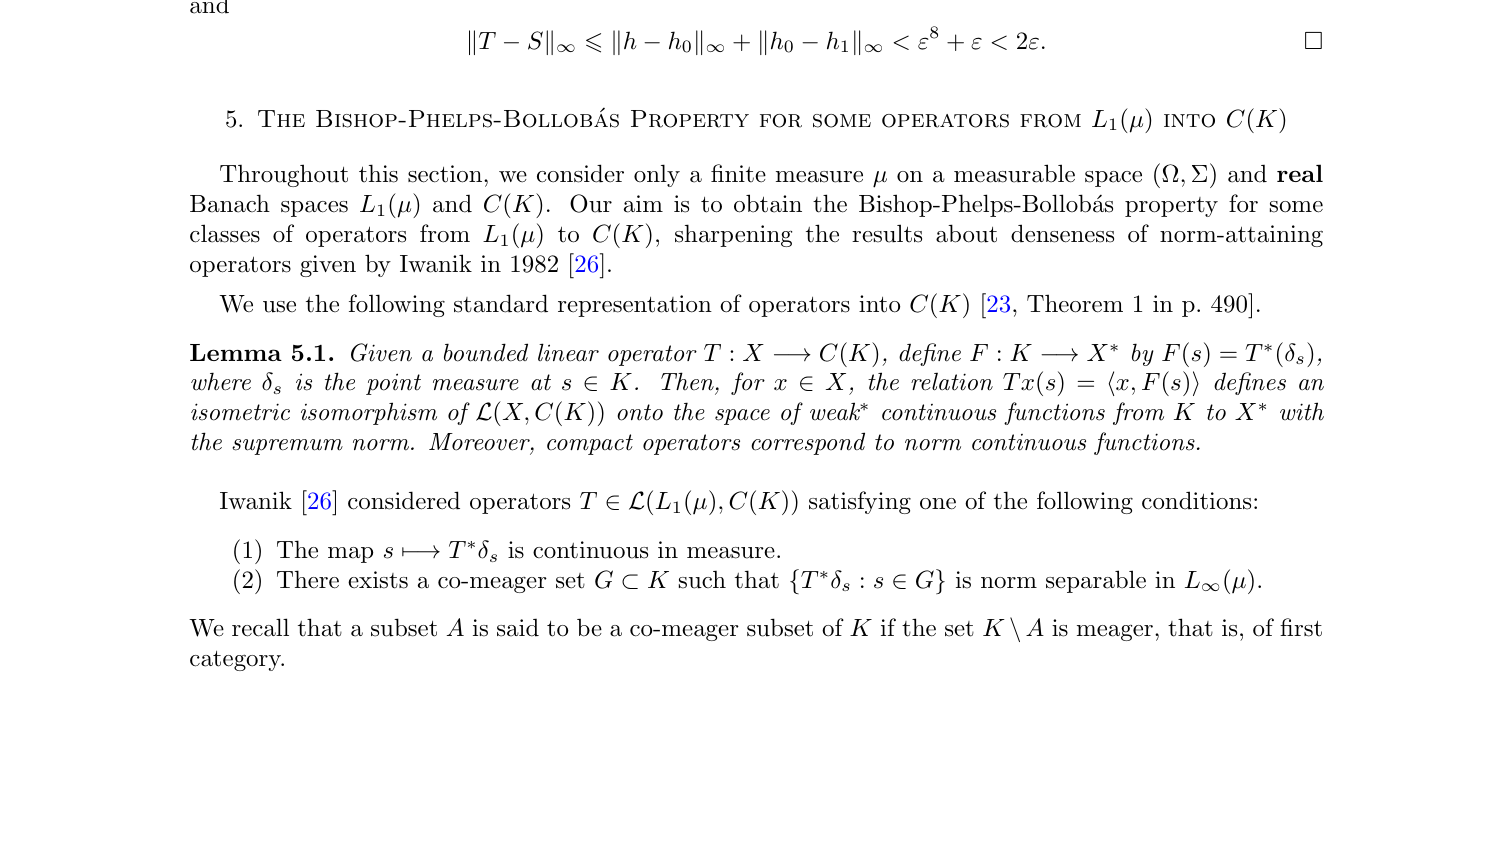
\includegraphics[width=0.96\textwidth]{figures/condition_context_crop.png}
\end{center}

Immediately after Theorem 5.2, on printed/PDF page 16, the authors ask:
\begin{quote}
``For which topological compact Hausdorff spaces $K$ all operators in
$\mathcal L(L_1(\mu),C(K))$ satisfy condition (1)?''
\end{quote}
The exact source passage is reproduced here:
\begin{center}

\includegraphics[width=0.96\textwidth]{figures/open_problem_crop.png}
\end{center}

We answer the question for each fixed finite measure $\mu$.  ``Purely
atomic'' always means modulo null sets.  This includes the zero measure.

\section{Proof intuition}

The map $F_T$ is automatically weak-star continuous: $s\mapsto\delta_s$ is
weak-star continuous in $C(K)^*$, and $T^*$ is weak-star to weak-star
continuous.  The question is therefore when every bounded weak-star
continuous field $F:K\to\Linfty$ must also be continuous in measure.

For a purely atomic measure, weak-star continuity gives scalar continuity on
each atom.  Only finitely many atoms are needed to cover all but an
arbitrarily small measure, so finitely many scalar estimates imply
continuity in measure.

On a nonatomic set, by contrast, the Rademacher functions are weak-star null
in $L_\infty$ but remain a fixed positive distance from zero in measure.
Every infinite compact Hausdorff space maps continuously onto an infinite
compact metric space, and such a space contains a nontrivial convergent
sequence.  Continuous scalar bumps around that sequence let us install the
Rademacher functions as the values of one weak-star continuous field.  The
field, and hence the corresponding operator, fails condition (1).

\section{Three lemmas}

\begin{lemma}[Operator--field correspondence]\label{lem:field}
For a bounded map $F:K\to\Linfty$, the following are equivalent:
\begin{enumerate}
\item $F$ is weak-star continuous;
\item there is a bounded operator $T:\Lone\to C(K)$ satisfying
      $T^*\delta_s=F(s)$ for every $s\in K$.
\end{enumerate}
In this case one may take
\[
 (Tf)(s)=\int fF(s)\,d\mu.
\]
\end{lemma}

\begin{proof}
Weak-star continuity makes the displayed scalar function continuous for
each $f\in\Lone$, and boundedness of $F$ gives a bounded operator.  The
identity for its adjoint follows directly from the definition.  Conversely,
for a given $T$, each pairing
$\langle F_T(s),f\rangle=(Tf)(s)$ is continuous, which is precisely
weak-star continuity.
\end{proof}

\begin{lemma}[An infinite metrizable image]\label{lem:image}
Every infinite compact Hausdorff space $K$ has an infinite compact metrizable
continuous image.
\end{lemma}

\begin{proof}
For $m\ge1$, let
\[
 \mathcal C_m=\{f\in C(K,\mathbb R): |f(K)|\le m\}.
\]
Each $\mathcal C_m$ is closed in the uniform norm: if a limit had $m+1$
distinct values, their positive minimum separation would force all
sufficiently close approximants to have at least $m+1$ values.

It also has empty interior.  Indeed, if $f\in\mathcal C_m$, one of its
finitely many level sets is infinite.  Choose $m+1$ distinct points in that
level set.  Since compact Hausdorff spaces are normal, the Tietze extension
theorem supplies an arbitrarily small real continuous perturbation taking
distinct prescribed values at those points.  The perturbed function is not
in $\mathcal C_m$.

The Banach space $C(K,\mathbb R)$ is a Baire space, so it is not the union of
the closed nowhere-dense sets $\mathcal C_m$.  Hence some
$\pi\in C(K,\mathbb R)$ has infinite range.  Then
$M=\pi(K)\subset\mathbb R$ is the required infinite compact metrizable
continuous image.
\end{proof}

\begin{lemma}[A weak-star/measure discontinuity]\label{lem:rademacher}
Suppose that $\mu$ has a nonatomic measurable part $E$ of positive measure.
There is a sequence $(r_n)$ in the unit ball of $\Linfty$ such that
$r_n\to0$ weak-star, while
\[
 \mu\bigl(\{|r_n|>1/2\}\bigr)=\mu(E)>0\qquad(n\ge1).
\]
\end{lemma}

\begin{proof}
Recursively bisect $E$ into measurable sets of equal measure.  On $E$, let
$r_n$ equal $1$ or $-1$ according to which half is selected at the $n$th
level of this dyadic partition, and put $r_n=0$ off $E$.  The displayed
measure identity is immediate.

Let $\mathcal A_n$ be the finite sigma-algebra generated by the first $n$
levels, and let $\mathcal A=\sigma(\bigcup_n\mathcal A_n)$.  For
$f\in\Lone$, conditional expectation gives
\[
 \int_E fr_n\,d\mu
 =\int_E \mathbb E(f\mid\mathcal A)r_n\,d\mu.
\]
The martingale convergence theorem approximates
$\mathbb E(f\mid\mathcal A)$ in $L_1$ by
$\mathbb E(f\mid\mathcal A_N)$.  For $n>N$, the latter has integral zero
against $r_n$.  Since $\|r_n\|_\infty\le1$, it follows that
$\int fr_n\,d\mu\to0$.  Thus $r_n\to0$ weak-star.
\end{proof}

\section{Complete classification}

\begin{theorem}\label{thm:main}
Let $\mu$ be a finite measure and $K$ a compact Hausdorff space.  Every
operator $T:L_1(\mu)\to C(K)$ satisfies condition (1) of
Choi--Kim--Lee--Mart\'in if and only if
\begin{equation}\label{eq:classification}
 \mu\text{ is purely atomic}\quad\text{or}\quad K\text{ is finite}.
\end{equation}
Equivalently, if $\mu$ has a nonatomic part, the admissible compacta are
exactly the finite ones; if $\mu$ is purely atomic, every compactum is
admissible.
\end{theorem}

\begin{proof}
First suppose that $K$ is finite.  It is discrete, so every map from $K$ is
continuous and condition (1) is automatic.

Now suppose that $\mu$ is purely atomic.  A finite purely atomic measure has
at most countably many positive-measure atoms $A_j$, and these cover the
space modulo a null set.  Every element of $\Linfty$ is essentially constant
on each $A_j$.  If $F=F_T$ and $c_j(s)$ denotes its value on $A_j$, then
\[
 c_j(s)=\frac1{\mu(A_j)}
 \left\langle F(s),\mathbf 1_{A_j}\right\rangle.
\]
Consequently every $c_j$ is continuous by weak-star continuity of $F$.

Fix $s_0\in K$ and positive $a,\varepsilon$.  Choose finitely many atoms
$A_1,\dots,A_N$ whose complement has measure less than $\varepsilon$.
For $s$ in a sufficiently small neighborhood of $s_0$,
$|c_j(s)-c_j(s_0)|\le a$ for $1\le j\le N$.  Therefore
\[
 \mu\bigl(\{|F(s)-F(s_0)|>a\}\bigr)<\varepsilon.
\]
This is continuity in measure.

It remains to prove necessity when $\mu$ has a nonatomic part and $K$ is
infinite.  By Lemma~\ref{lem:image}, choose a continuous surjection
$\pi:K\to M$ onto an infinite compact metric space.  There are distinct
points $t_n,t_0\in M$ with $t_n\to t_0$.  Passing to a subsequence, choose
pairwise disjoint open sets $U_n$ containing $t_n$, whose closures avoid
$t_0$ and whose union accumulates only at $t_0$.  By normality, choose
$\varphi_n\in C(M,[0,1])$ with
\[
\varphi_n(t_n)=1,\qquad
 \operatorname{supp}\varphi_n\subset U_n.
\]

Take the sequence $(r_n)$ from Lemma~\ref{lem:rademacher} and define
\[
 F_0(t_0)=0,\qquad
 F_0(t)=\sum_{n=1}^\infty \varphi_n(t)r_n\quad(t\in M).
\]
At most one term is nonzero, so $\|F_0(t)\|_\infty\le1$.  Away from $t_0$
the field is locally either zero or a scalar multiple of one fixed $r_n$,
and is therefore norm-continuous.  At $t_0$, fix $f\in\Lone$.  Since
$\langle r_n,f\rangle\to0$, all sufficiently late bumps have uniformly
small pairing with $f$; a neighborhood of $t_0$ misses the finitely many
early supports.  Thus
$\langle F_0(t),f\rangle\to0$ as $t\to t_0$.  Hence $F_0$ is weak-star
continuous on $M$.

Set $F=F_0\circ\pi$.  Lemma~\ref{lem:field} produces
$T:\Lone\to C(K)$ with $F_T=F$.  Choose $s_n\in K$ with
$\pi(s_n)=t_n$.  Compactness gives a convergent subnet
$s_{n_\alpha}\to s_0$, and continuity of $\pi$ forces
$\pi(s_0)=t_0$.  But
\[
 F(s_{n_\alpha})=r_{n_\alpha},\qquad F(s_0)=0,
\]
and Lemma~\ref{lem:rademacher} shows that this subnet does not converge in
measure.  Thus $F_T$ is not continuous in measure.  This constructs a
counterexample whenever both alternatives in \eqref{eq:classification}
fail.
\end{proof}

\section{Verification, scope, and novelty audit}

The construction is qualitative but every logical interface can be checked
directly:
\begin{enumerate}
\item Lemma~\ref{lem:field} verifies that no representability assumption on
      the weak-star continuous field is missing.
\item The Baire argument in Lemma~\ref{lem:image} avoids any false
      sequentiality claim about a general compact Hausdorff $K$; only its
      metrizable image is used to choose a sequence.
\item Lemma~\ref{lem:rademacher} proves weak-star nullity for every
      $f\in L_1(\mu)$, not merely for dyadic simple functions.
\item A convergent subnet of the chosen lifts transfers the failure of
      measure convergence back from $M$ to $K$.
\end{enumerate}

The theorem concerns the fixed finite measure appearing in the source
question.  It does not assert a uniform statement over all measures, nor
does it decide when condition (1) is equivalent to the Bishop--Phelps--Bollob\'as
property in settings outside the hypotheses of the source paper.

The bounded novelty search checked the run's solution, attempt, proof-gap,
and ledger indexes; the parsed local arXiv corpus; exact arXiv-id and title
queries; the exact question; and close searches combining ``Iwanik'',
``condition (1)'', weak-star continuity, convergence in measure, atomic
measures, and compact Hausdorff spaces.  It also checked later citations and
closely related Bishop--Phelps--Bollob\'as papers returned by those searches.
No later paper stating this dichotomy was found.  That is evidence of
novelty, not an exhaustive literature guarantee.

Human review should prioritize Lemma~\ref{lem:image} and weak-star
continuity of $F_0$ at $t_0$.  No computer algebra or numerical experiment is
used.

\begin{thebibliography}{9}
\bibitem{CKLM}
Y.~S. Choi, S.~K. Kim, H.~J. Lee, and M.~Mart\'in,
\emph{The Bishop--Phelps--Bollob\'as theorem for operators on $L_1(\mu)$},
Journal of Functional Analysis \textbf{267} (2014), 214--242;
arXiv:1303.6078; doi:10.1016/j.jfa.2014.04.008.

\bibitem{Bogachev}
V.~I. Bogachev, \emph{Measure Theory}, Vol.~I, Springer, 2007.

\bibitem{Engelking}
R.~Engelking, \emph{General Topology}, 2nd ed., Heldermann, 1989.
\end{thebibliography}

\end{document}
